\documentclass{beamer} 

\usepackage{graphicx}
\usepackage{subfigure}

%\usepackage{xeCJK} % 中文包
\usetheme{Boadilla}  
\usecolortheme{seagull} 

%\setbeamertemplate{caption}[numbered] % 序号
%\setbeamercovered{transparent=15}
\setbeamersize{text margin left=0.6cm, text margin right=0.6cm} % 设置页边距
\setbeamercovered{transparent} 
\setbeamertemplate{navigation symbols}{} %Navigationsleiste ausschalten     


\title{Weekly work summary}
\author{Guangzhi Ren}
\institute {}
\date{\today}

\begin{document}
	
\begin{frame}
	\titlepage   
\end{frame}


\begin{frame}{content}
\begin{itemize}
	\item revisiting to former simulation result
	\item spectral simulation base on electromagnetic 5-field landau fluid
		\begin{itemize}
%			\item parallel computation scheme
%			\item comparision between different algorithms
			\item conservation test
			\item initial perturbation
%			\item residual flow simulation
		\end{itemize}
%	\item residual flow and GAM
%	\item Hammett-Perkins closure 	
\end{itemize}
\end{frame}



\begin{frame}{revisiting to former simulation result}
	\begin{figure}[H]
		\centering
		\subfigure[$\beta=0.1\%$]{
			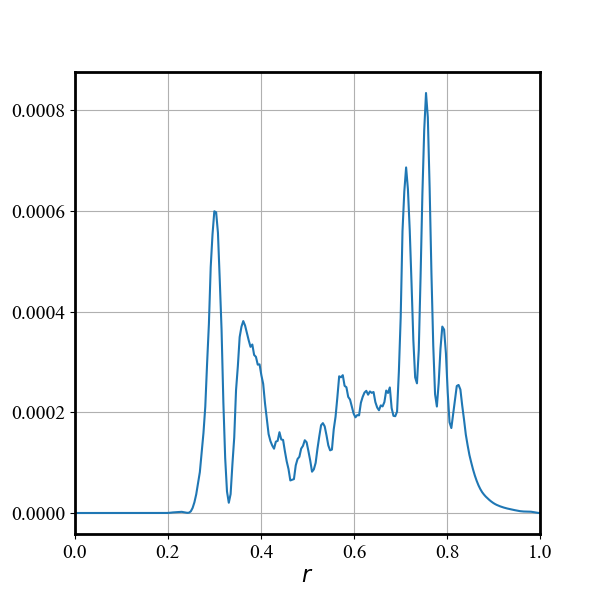
\includegraphics[width=0.2\textwidth]{./images/Ezfx_b01.png} 
		}
		\subfigure[$\beta=0.3\%$]{
			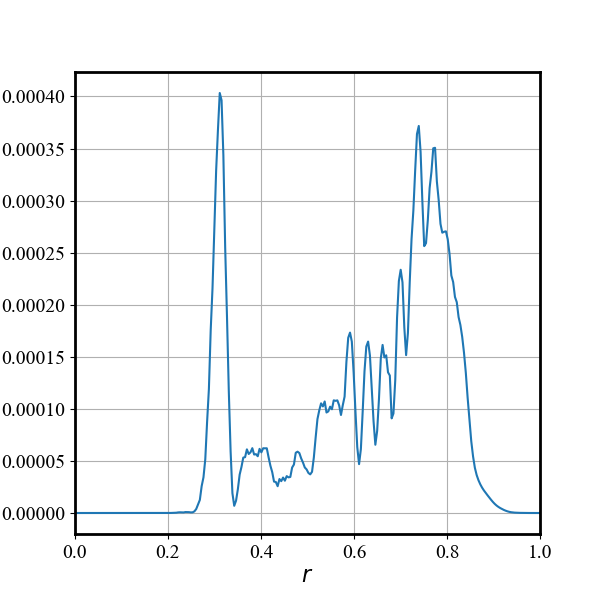
\includegraphics[width=0.2\textwidth]{./images/Ezfx_b03.png}
		}
		\subfigure[$\beta=1.0\%$]{
			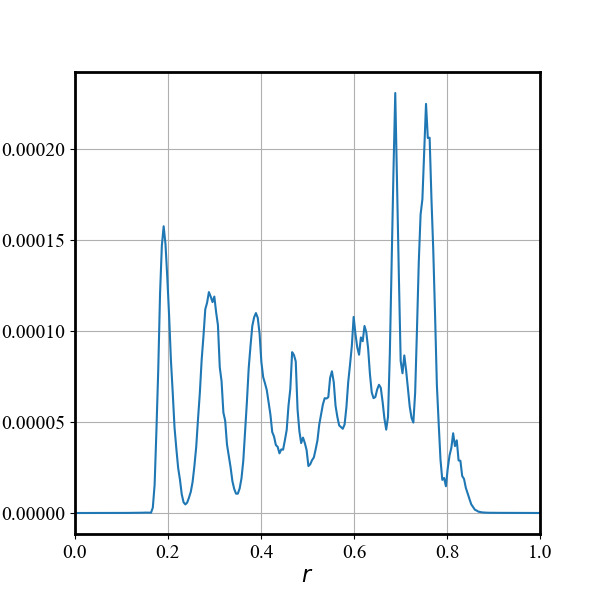
\includegraphics[width=0.2\textwidth]{./images/Ezfx_b10.png}
		}
		\subfigure[$\beta=1.2\%$]{
			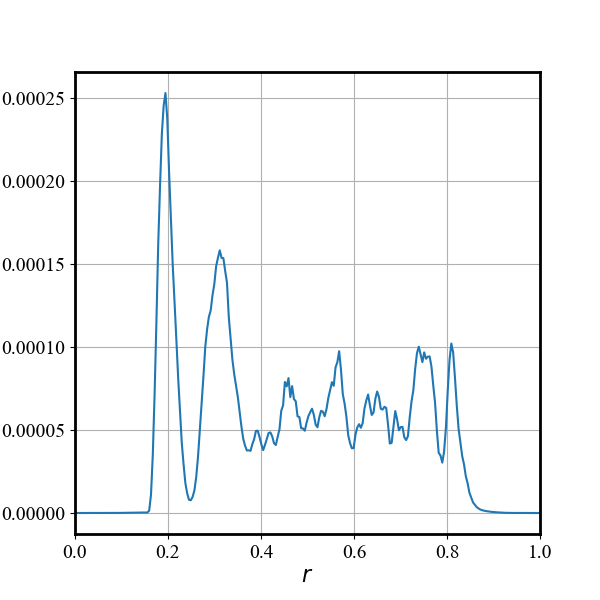
\includegraphics[width=0.2\textwidth]{./images/Ezfx_b12.png}
		}
		\caption{ Time averaged zonal flow profile }
	\end{figure}
	
\end{frame}



\begin{frame}{revisiting to former simulation result}
	\begin{figure}[H]
		\centering
		\subfigure[$\beta=0.1\%$]{
			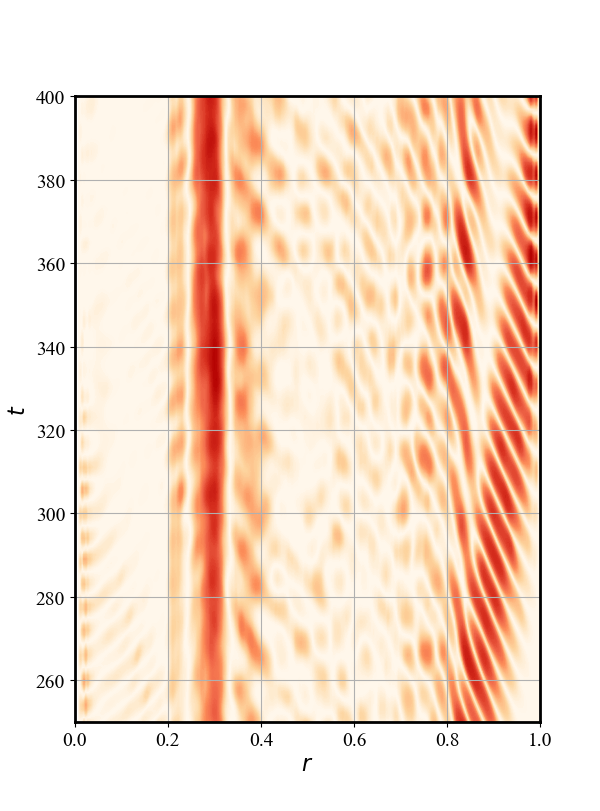
\includegraphics[width=0.2\textwidth]{./images/Ezf_b01.png} 
		}
		\subfigure[$\beta=0.3\%$]{
			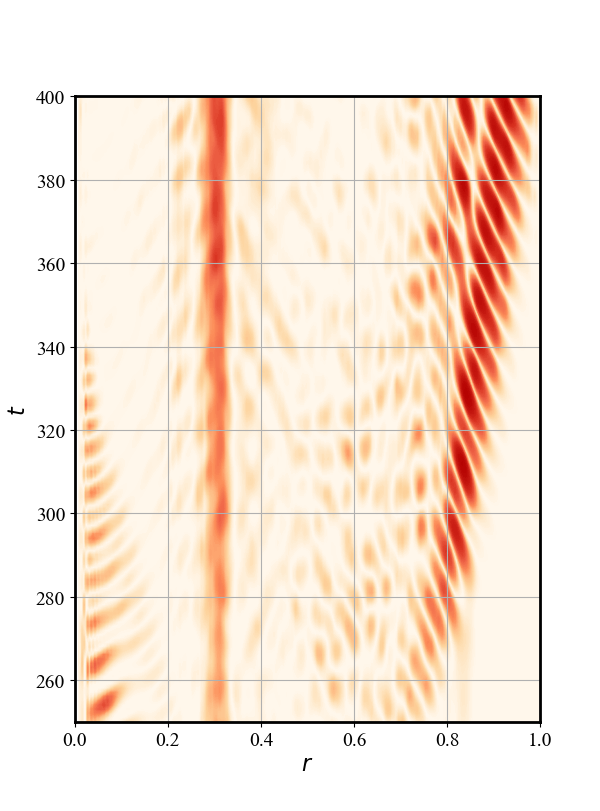
\includegraphics[width=0.2\textwidth]{./images/Ezf_b03.png}
		}
		\subfigure[$\beta=1.0\%$]{
			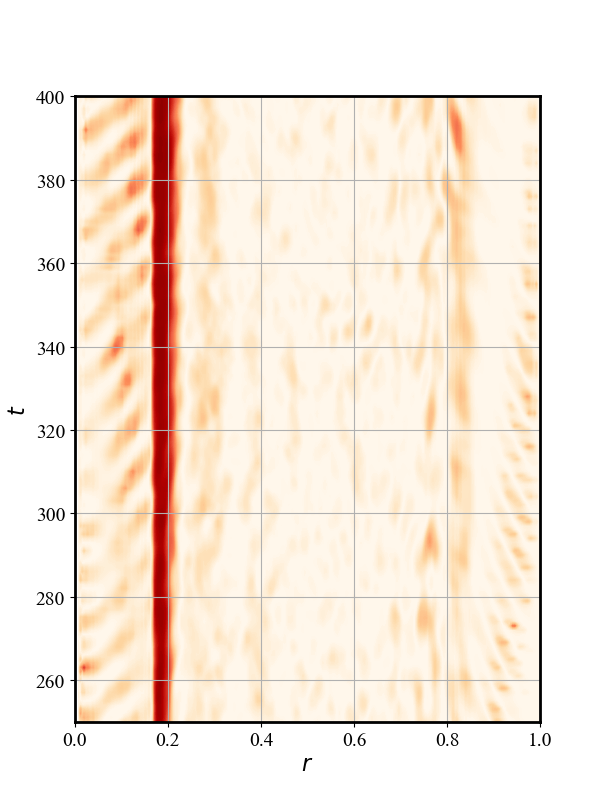
\includegraphics[width=0.2\textwidth]{./images/Ezf_b10.png}
		}
		\subfigure[$\beta=1.2\%$]{
			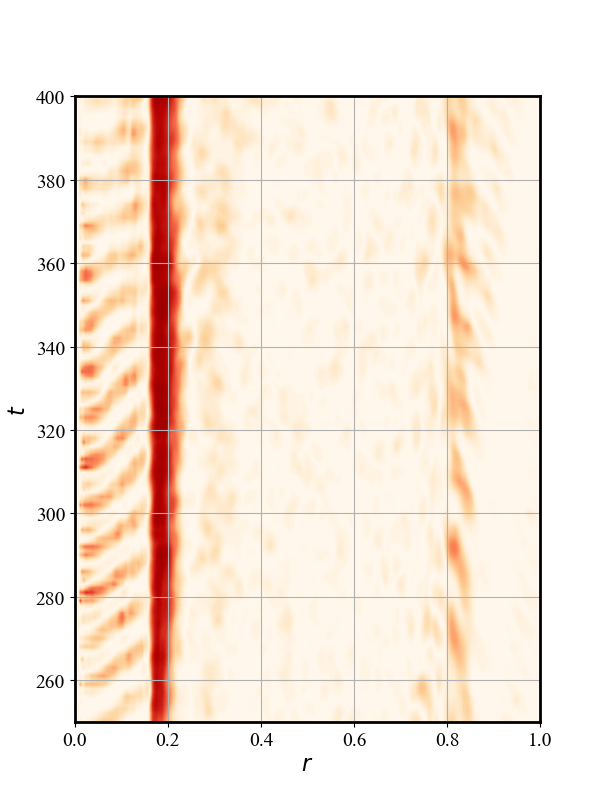
\includegraphics[width=0.2\textwidth]{./images/Ezf_b12.png}
		}
		\caption{ The ratio $E_{zf}/E_{total}$ as a function of radius and time }
	\end{figure}

	Maybe a low q profile should be selected to check the results.
\end{frame}




\begin{frame}{consevation test}

\begin{figure}[H]
	\centering
	\subfigure[$\beta=0.1\%$]{
		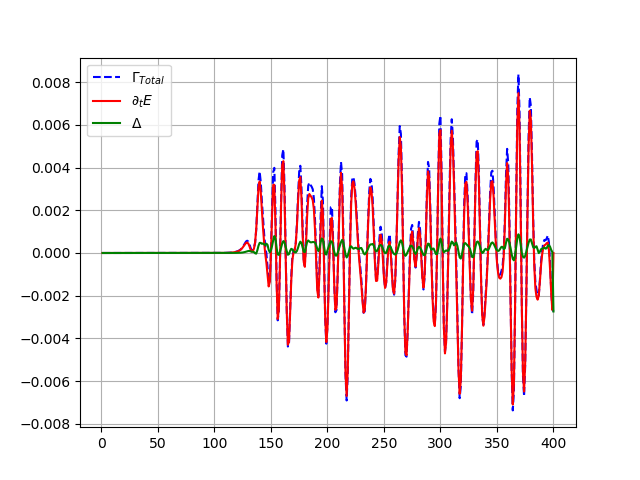
\includegraphics[width=0.4\textwidth]{./images/zft_b01.png} 
	}
	\subfigure[$\beta=1.0\%$]{
		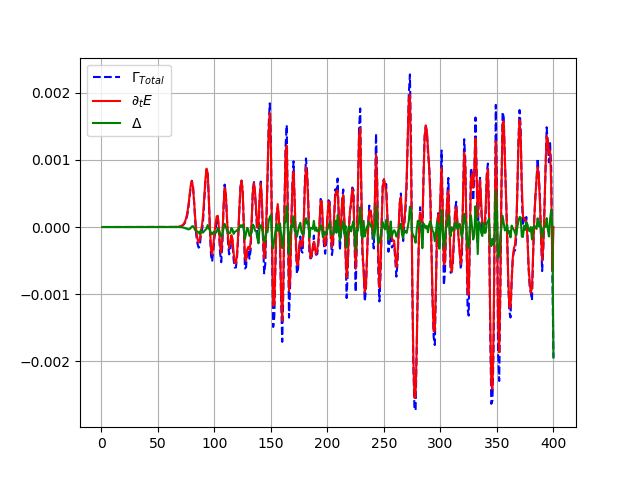
\includegraphics[width=0.4\textwidth]{./images/zft_b10.png}
	}
	\caption{derivative of zonal flow energy }
\end{figure}

	\begin{quotation}
		{\color{magenta} question:\ accuration}
	\end{quotation}

\end{frame}


\begin{frame}{consevation test}
	for LW2: 
	\begin{equation}
		\frac{f_x^t-f_x^{t-\Delta{t}}}{\Delta{t}}-\mu(\nabla_\perp^2{f})_x^{t}
		= \frac{1}{2}( C_{x-1/2}^{t-\Delta{t}/2}+C_{x+1/2}^{t-\Delta{t}/2} )
	\end{equation}
	
	\begin{equation}
		\frac{E_x^t-E_x^{t-\Delta{t}}}{\Delta{t}}
		= \mathcal{E}\{ \frac{1}{2}( C_{x-1/2}^{t-\Delta{t}/2}+C_{x+1/2}^{t-\Delta{t}/2} ) +\mu(\nabla_\perp^2{f})_x^{t} \}
	\end{equation}
	
	\begin{quotation}
		{\color{blue} problem:\ deviation triggered by volumn integration}
	\end{quotation}
	another idea:	\\
	\qquad $E$ as a coupling equation to field equation set
\end{frame}


\begin{frame}{consevation test}
	\begin{figure}[H]
	\centering
	\subfigure[$f\sim f(t-\Delta{t}/2)$]{
		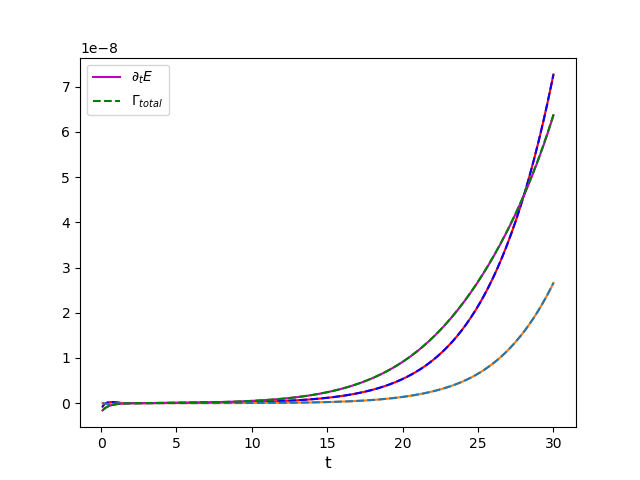
\includegraphics[width=0.4\textwidth]{./images/cons_lw.png} 
	}
	\subfigure[$f\sim f(t)$]{
		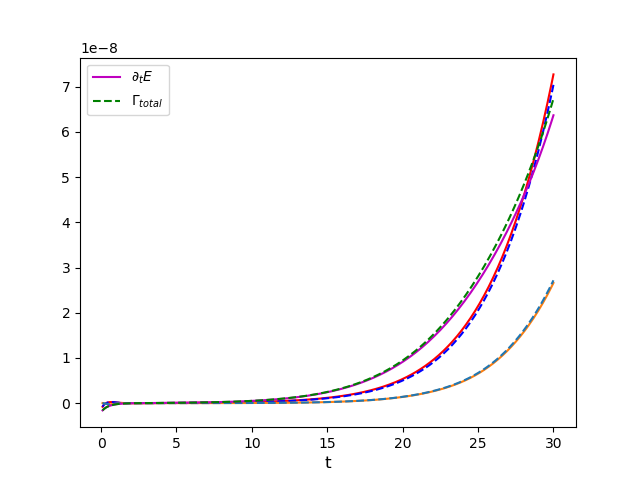
\includegraphics[width=0.4\textwidth]{./images/cons_lw_02.png}
	}
	\caption{ derivative of energy with LW2 }
	\end{figure}
\end{frame}


\begin{frame}{consevation test}
	
	\begin{figure}[H]
		\centering
		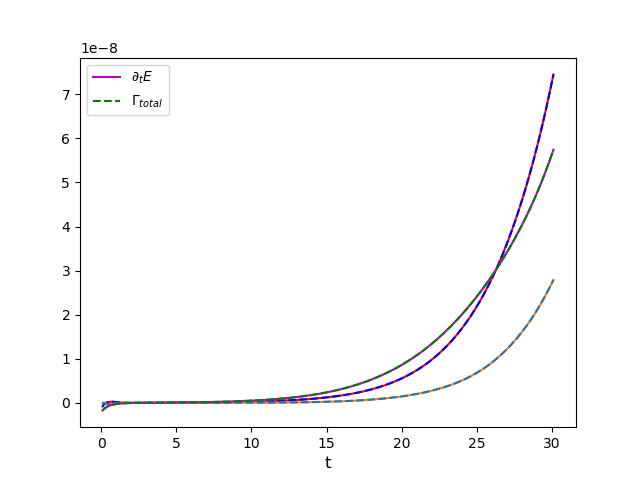
\includegraphics[width=0.5\textwidth]{./images/cons_ab.png}
		\caption{derivative of energy with AB2}
	\end{figure}
\end{frame}


\begin{frame}{initial perturbation}
	\begin{figure}[H]
		\centering
		\subfigure{
			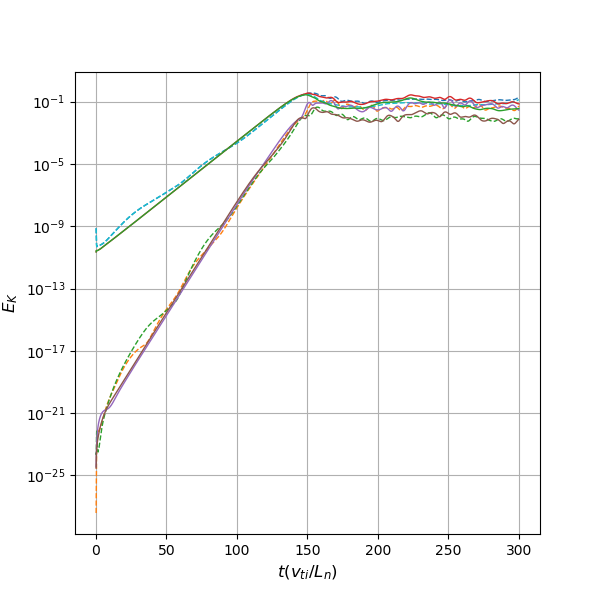
\includegraphics[width=0.4\textwidth]{./images/ini_E_01.png} 
		}
		\subfigure{
			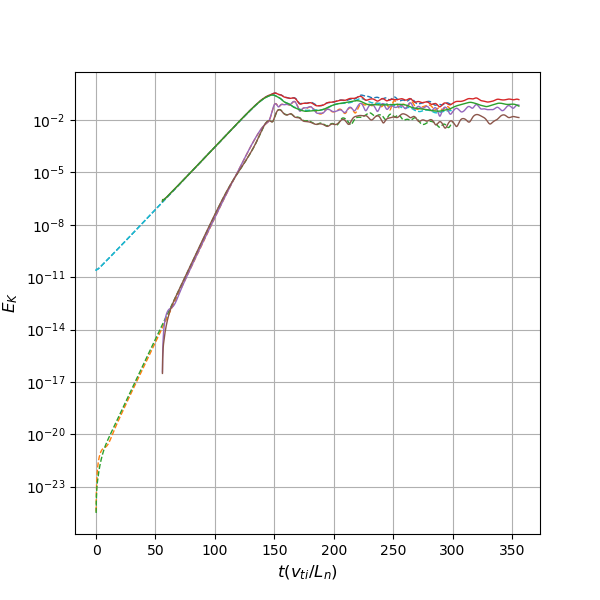
\includegraphics[width=0.4\textwidth]{./images/ini_E_02.png}
		}
		\caption{ evolution of kinetic energy with different initial perturbation }
	\end{figure}
\end{frame}


\end{document}